\documentclass{beamer}
\mode<presentation>
{
  \usetheme{Warsaw}
  \definecolor{utorange}{rgb}{1.0, 0.5098, 0}
  \definecolor{utwhite}{rgb}{1.0, 1.0, 1.0}
  \setbeamercolor{structure}{fg=utorange,bg=utwhite}
  \setbeamertemplate{frametitle}[default][shadow=false]
  %\setbeamercovered{transparent}
}


%\mode
%<handout>
%\usepackage{pgfpages}
%\pgfpagesuselayout{4 on 1}[letterpaper,border shrink=4mm]
%\setbeamertemplate{footline}[page number]



\usepackage[english]{babel}
\usepackage[latin1]{inputenc}
\usepackage{times}
\usepackage[T1]{fontenc}
\usepackage{tikz}
\usepackage{graphicx}
\usepackage[]{algorithm2e}
\usepackage{subfig}

\newcommand{\imagesource}[1]{{\centering\hfill\break\hbox{\scriptsize Image Source:\thinspace{\small\itshape #1}}\par}}

\title{Influence Modeling With Tensors}


\author{Robert Lowe - robert.lowe@maryvillecollege.edu}

\date[]{}
\subject{}

\pgfdeclareimage[height=0.5cm]{university-logo}{images/utklogo}
\logo{\pgfuseimage{university-logo}}



\AtBeginSection[]
{
  \begin{frame}<beamer>{Outline}
    \tableofcontents[currentsection]
  \end{frame}
}


\begin{document}

\begin{frame}
  \titlepage
\end{frame}

\begin{frame}{Outline}
  \tableofcontents
\end{frame}


% Structuring a talk is a difficult task and the following structure
% may not be suitable. Here are some rules that apply for this
% solution: 

% - Exactly two or three sections (other than the summary).
% - At *most* three subsections per section.
% - Talk about 30s to 2min per frame. So there should be between about
%   15 and 30 frames, all told.

% - A conference audience is likely to know very little of what you
%   are going to talk about. So *simplify*!
% - In a 20min talk, getting the main ideas across is hard
%   enough. Leave out details, even if it means being less precise than
%   you think necessary.
% - If you omit details that are vital to the proof/implementation,
%   just say so once. Everybody will be happy with that.

\section{Introduction}
\begin{frame}{Problem Statement}
    \begin{columns}
        \column{0.5\textwidth}
        Evaluating Citations by Influence Modeling
        \begin{itemize}[<+->]
            \item What sort of impact does an author have?
            \item Are claimed citations valid?
            \item Are there missing citations?
            \item Which document came first?
        \end{itemize}
        \column{0.5\textwidth}
        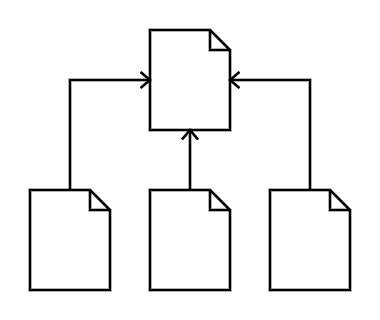
\includegraphics[width=\textwidth]{images/Citations}
    \end{columns}
\end{frame}

\begin{frame}{Related Work}
    \begin{itemize}[<+->]
        \item {\em Citation Statistics}. Adler, Ewing, and Taylor (2009)
            \par Indicates the need for better citation metrics.\cite{adler2009}
        \item {\em Unsupervised prediction of citation influences}.  Dietz, Bickel, Scheffer. (2007)\cite{dietz2007}
            \par LDA Based directed graph influence model.
        \item {\em Beyond Keyword Search: Discovering Relevant Scientific Literature}. El-Arini and Guestrin. (2011)\cite{el-arini2011}
            \par Presents a keyword frequency based influence model used to search for relevant documents.
    \end{itemize}
\end{frame}


\section{Approach}

\begin{frame}{Overview}
    \begin{enumerate}[<+->]
        \item Model all documents in a corpus as tensors.
        \item Decompose the tensors into rank-1 factors.
        \item Assign weights to each factor by comparing cited factors with the factors of the citing document.
        \item Adjust weights to determine overall influence of documents and authors.
    \end{enumerate}
\end{frame}

\begin{frame}{Tensors}
    \begin{columns}
        \column{0.5\textwidth}
        \begin{itemize}[<+->]
            \item A tensor can have any number of {\bf modes}, each corresponding to a variable.
            \item Frequently tensors are depicted as having 3 modes, but they can be of any dimension.
            \item A tensor's {\bf rank} is the minimal number of modes needed to represent a tensor.
        \end{itemize}
        \column{0.5\textwidth}
        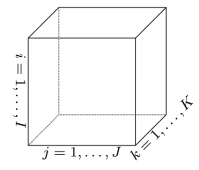
\includegraphics[width=\textwidth]{images/tensor}
        \imagesource{Rasmus Bro 1997~\cite{bro1997}}
    \end{columns}
\end{frame}

\begin{frame}{PARAFAC}
    \begin{center}
    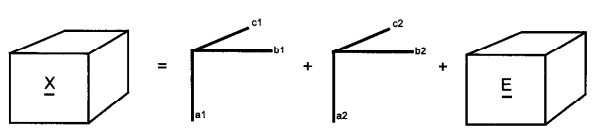
\includegraphics[height=0.20\textheight]{images/parafac}
    \imagesource{Rasmus Bro 1997~\cite{bro1997}}
    \end{center}
    \begin{itemize}[<+->]
        \item Popularized by Richard Harshman \cite{harshman1970} as a means of analyzing multi-modal parallel factors.
        \item Decomposes a tensor as a sum of component tensors.
        \item The component tensors are represented as a set of loading vectors such that the tensor $T$ is created by:
        \[
    T = \displaystyle\sum_{i=1}^{r} \lambda_i A_i \circ B_i \circ C_i + E
        \]
    \end{itemize}
\end{frame}

\begin{frame}{Selecting Number of Factors}
    \begin{itemize}[<+->]
        \item PARAFAC is unique under rotation so long as the number of factors is greater than or equal to the rank of the tensor.
        \item Tensor rank is np-complete (Haastad 1990)\cite{haastad1990}
        \item An approximation of the optimal number of factors can be approximated using techniques such as CORCONDIA (Bro 2003) \cite{bro2003}.
        \item CORCONDIA checks the core consistency of the model by repeatedly dividing by the factors of the tensor.
        \item Consistent models should result in superdiagonal core tensor.
    \end{itemize}
\end{frame}

\begin{frame}{Document Model}
    \begin{itemize}[<+->]
        \item Corpus vocabulary $vocab$
        \item Tensors for each document which are $|vocab| \times |vocab| \times \ldots \times |vocab|$ in dimension.
        \item Tensor elements count n-gram frequencies where $n$ is the number of dimensions
    \end{itemize}
\end{frame}

\begin{frame}{Corpus Preparation}
\begin{algorithm}[H]
    Remove Numbers\;
    Remove Punctuation\;
    $wl \leftarrow $ split all documents by spaces\;
    $vocab \leftarrow \emptyset$\;
    \For{$w$ in $wl$} {
        \If{$w \notin vocab$}{
            $vocab$.append($w$)\;
        }
    }
\end{algorithm}
\end{frame}

\begin{frame}{Document Model Construction}
\begin{algorithm}[H]
    $T \leftarrow$ 0 tensor with dimension $|vocab| \times |vocab| \times \ldots
    |vocab|$\;
    $phrase \leftarrow \emptyset$ \;
    \For{$w$ in $d$}{
        $phrase$.append($w$)\;
        \If{$|phrase| = n$}{
            $idx \leftarrow \emptyset$ \;
            \For{$p$ in $phrase$}{
                $i \leftarrow vocab.\mathrm{find}(p)$\;
                $idx.\mathrm{append}(i)$\;
            }
            $T[idx] \leftarrow T[idx] + 1$\;
        }
    }
\end{algorithm}
\end{frame}

\begin{frame}{Influence Model}
    \[
    C = \sum w_id_i + w_a A
    \]
    \begin{itemize}[<+->]
        \item $C$ - Citing Document Tensor
        \item $d_i$ - Factors of Cited Documents
        \item $w_i$ - Contribution Weight of Cited Factors
        \item $w_a$ - Weight of the author's contribution
        \item $A$ - Tensor representing the author's contribution
    \end{itemize}
\end{frame}

\begin{frame}{Weight Assignment}
\begin{algorithm}[H]
    $D \leftarrow$ PARAFAC decompositions of cited documents\;
    $F \leftarrow$ PARAFAC decomposition of citing document\;
    $\lambda_d \leftarrow $ Norms of Factors in $D$\;
    $\lambda_f \leftarrow $ Norms of Factors in $F$\;
    Normalize $D$ using $\lambda_d$\;
    Normalize $F$ using $\lambda_f$\;
    $w \leftarrow $ matrix of dimension $|D| \times |F|$\;
    \For{$i$ = 1 to $|D|$} {
        \For{$j$ = 1 to $|F|$} {
            $w[i,j] \leftarrow \mathrm{similarity(D[i], F[i])}$;
        }
    }
\end{algorithm}
\end{frame}

\begin{frame}{Similarity Measure - RMSD}
    As a place holder, the similarity measurement used in the example problem is
    root mean square deviation.
    \[
        \mathrm{RMSD}(X, Y) = \displaystyle\sqrt{\frac{1}{n}\sum(X_i - Y_i)^2}
    \]
\end{frame}

\begin{frame}{Factor Selection and Adjustment}
\begin{algorithm}[H]
    $indexes \leftarrow \emptyset$\;
    $weights \leftarrow \emptyset$\;
    \For{$c$ = 1 to $|F|$}{
        $i \leftarrow $ index of maximum weight in column $c$ of $w$\;
        $indexes.\mathrm{append}(i)$\;
        $weights.\mathrm{append}(w[i,c])$\;
    }
\end{algorithm}

\begin{algorithm}[H]
    $s \leftarrow \sum \lambda_f$\;
    \For{i = 1 to |w|} {
        $w[i] \leftarrow \lambda_f[i] * w[i] / s$\;
    }
\end{algorithm}

\end{frame}

\section{Example Problem}
\begin{frame}{Test Set Formulation}
    \begin{itemize}[<+->]
        \item To keep vocabulary small, children's' stories are used.
        \begin{itemize}
            \item {\em The Ant and the Dove} from Aesop's Fables~\cite{aesop}
            \item {\em The Seven Ravens} from Grimm's Fairy Tales~\cite{grimm}
        \end{itemize}
        \item A Markov Chain-Based Program (DadaDodo~\cite{dada}) generated a third document based on word probabilities learned from the source material.
        \item The resultant document is mostly nonsensical, but it does have a somewhat disturbing plot nonetheless!
        \begin{block}{}
But the glass, she the ring drumstick, of men! 

But a morsel from each of wings and looked at it was true that wish I am
looking for a little chair as he was once a human mouth. 
        \end{block}
    \end{itemize}
\end{frame}

\begin{frame}{Test Set Statistics}
    \begin{itemize}[<+->]
        \item 3 document corpus.
        \item 385 word vocabulary.
        \item 3-gram analysis is performed.
        \item {\em The Ant and the Dove} contributes 258 phrases.
        \item {\em The Seven Ravens} contributes 939 phrases.
        \item The generated document contains 619 phrases.
        \item CORCONDIA analysis indicates that 5 factors provides a good fit for all documents in the corpus.
    \end{itemize}
\end{frame}

\begin{frame}{Expected Document Contributions}
    \begin{columns}
        \column{0.5\textwidth}
        \begin{itemize}[<+->]
            \item The DadaDodo software draws evenly from both document.
            \item Because we are using Markov chaining, only next-word probabilities are used, hence the system can invent new phrases.
            \item The software invented 372 new phrases which appear in the generated documents.
        \end{itemize}
        \column{0.5\textwidth}
        \begin{tabular}{l|r}
        {\bf Document} & {\bf contribution} \\
        \hline
        Ant &  0.2261 \\
        Raven & 0.2261 \\
        $w_a$ & 0.54 \\
        \end{tabular}
    \end{columns}
\end{frame}

\begin{frame}{Results}
    \begin{tabular}{l|r}
        {\bf Source} & {\bf Contribution} \\
        \hline
        {\em The Ant and the Dove} & 0.24 \\
        {\em The Seven Ravens} & 0.22 \\
        $w_a$ & 0.54
    \end{tabular}
    \begin{itemize}[<+->]
        \item Contribution weights are close to expected results.
        \item The temporary factor matching, however, leaves much to be desired!
    \end{itemize}
\end{frame}

\begin{frame}{Factor 1 Match}
\begin{figure}%
    \centering
    \subfloat{{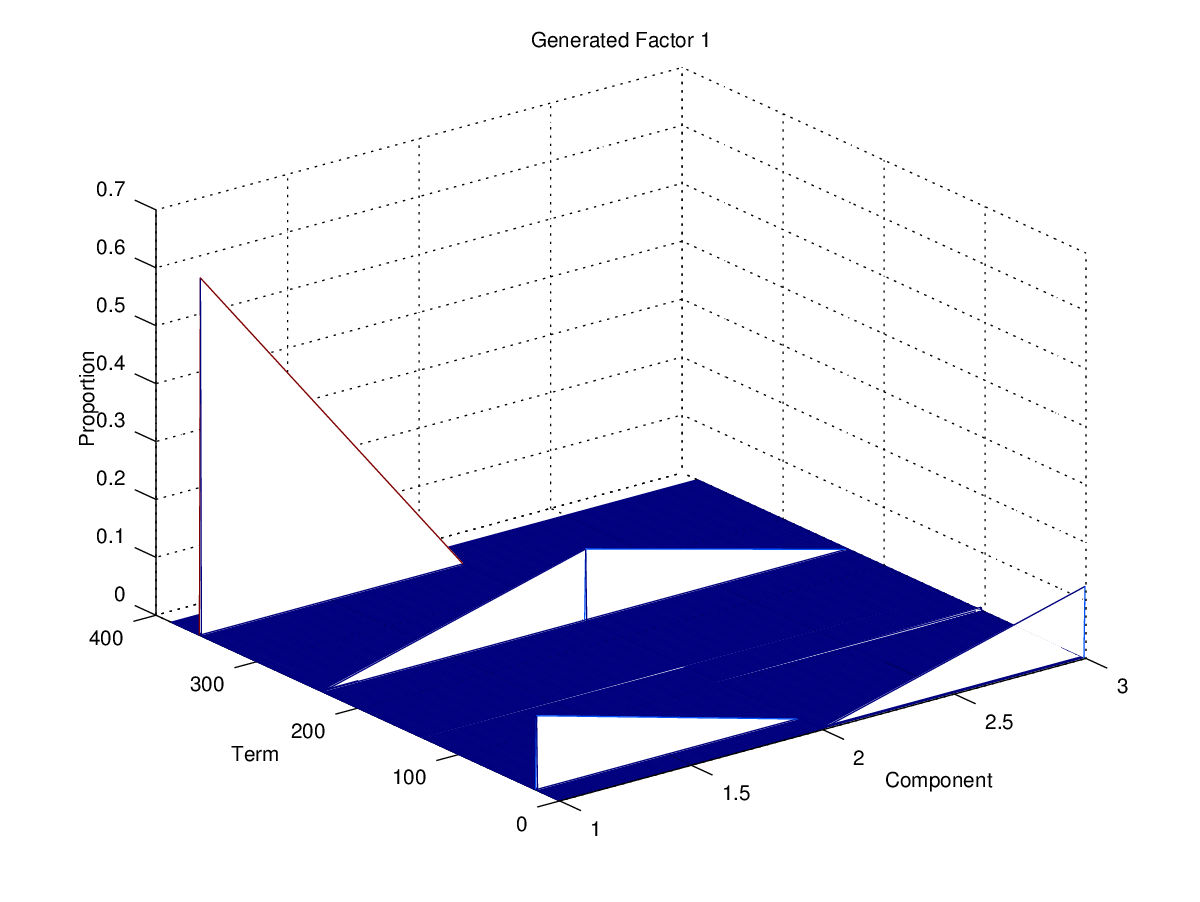
\includegraphics[width=0.4\textwidth]{plots/gen1} }}%
    \qquad
    \subfloat{{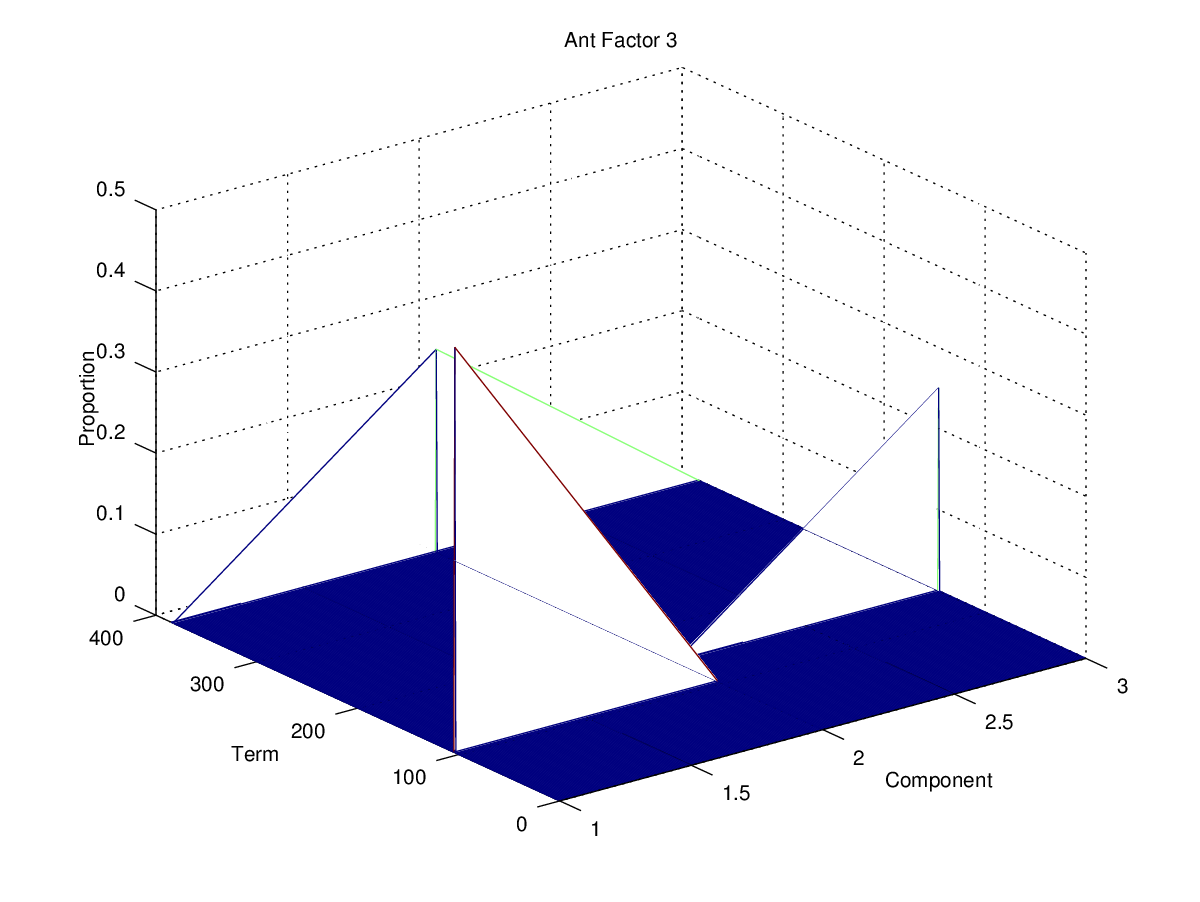
\includegraphics[width=0.4\textwidth]{plots/ant3}
    }}%
    \caption{Factor 1 Match}%
    \label{fig:com1}%
    Influence Source: Ant Factor 3 
    \par Influence Weight = 0.06
\end{figure}

\end{frame}

\begin{frame}{Factor 2 Match}
\begin{figure}%
    \centering
    \subfloat{{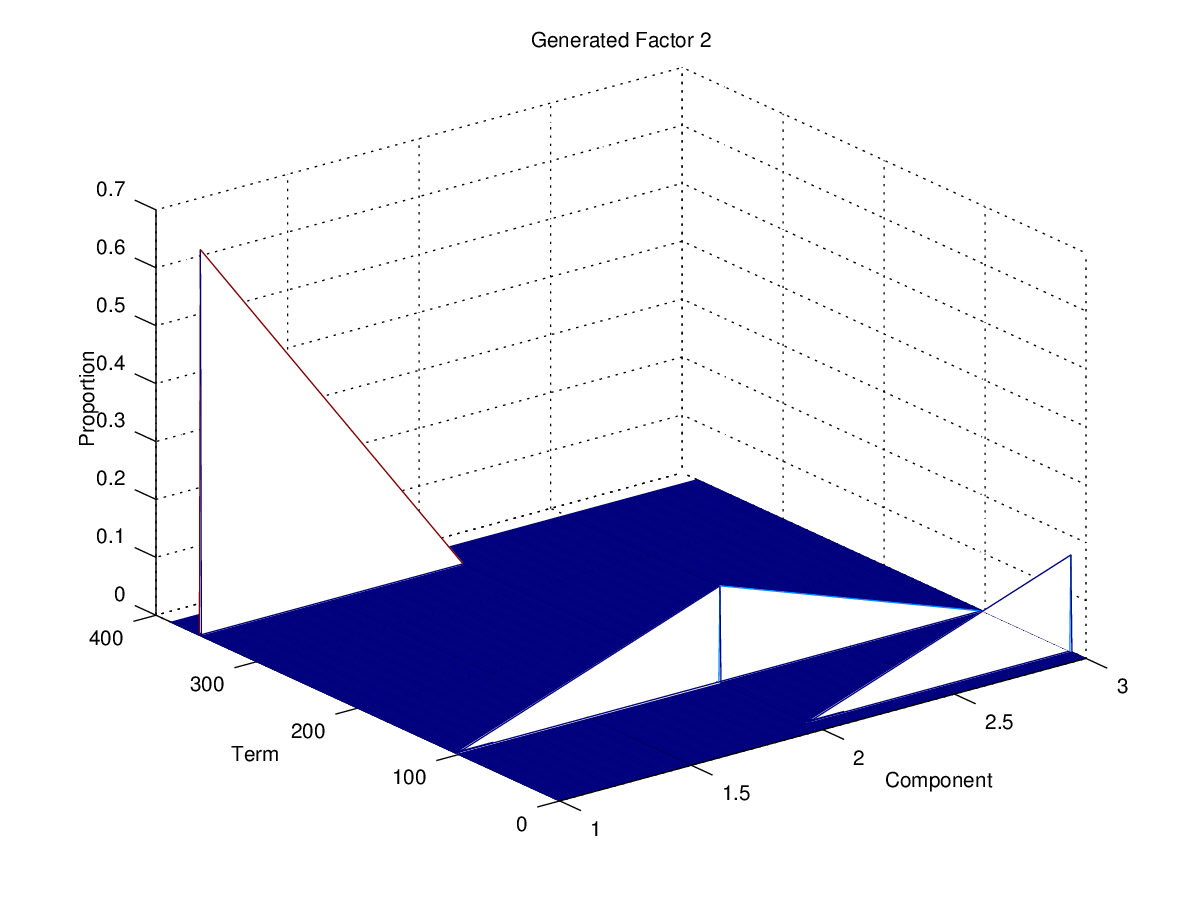
\includegraphics[width=0.4\textwidth]{plots/gen2} }}%
    \qquad
    \subfloat{{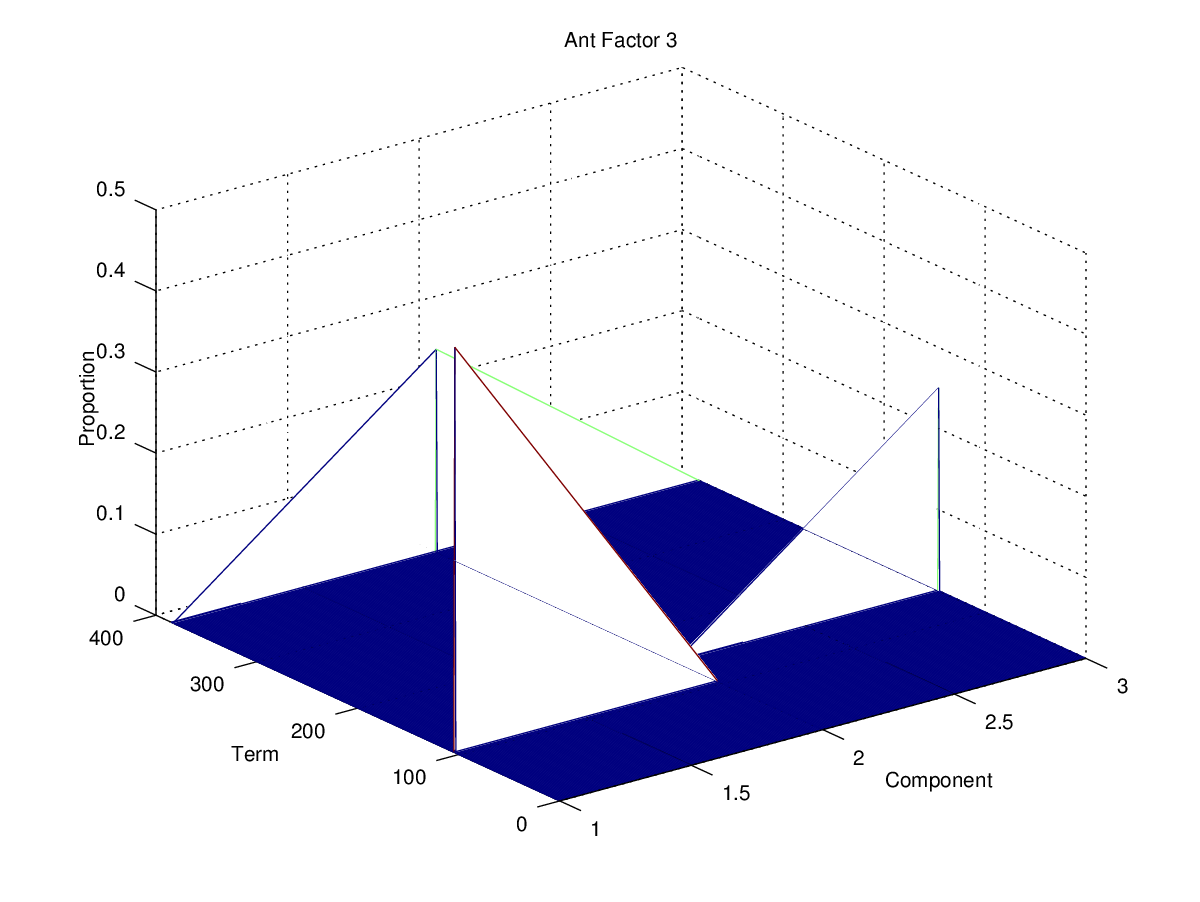
\includegraphics[width=0.4\textwidth]{plots/ant3}
    }}%
    \caption{Factor 2 Match}%
    \label{fig:com2}%
    Influence Source: Ant Factor 3 
    \par Influence Weight = 0.04
\end{figure}
\end{frame}

\begin{frame}{Factor 3 Match}
\begin{figure}%
    \centering
    \subfloat{{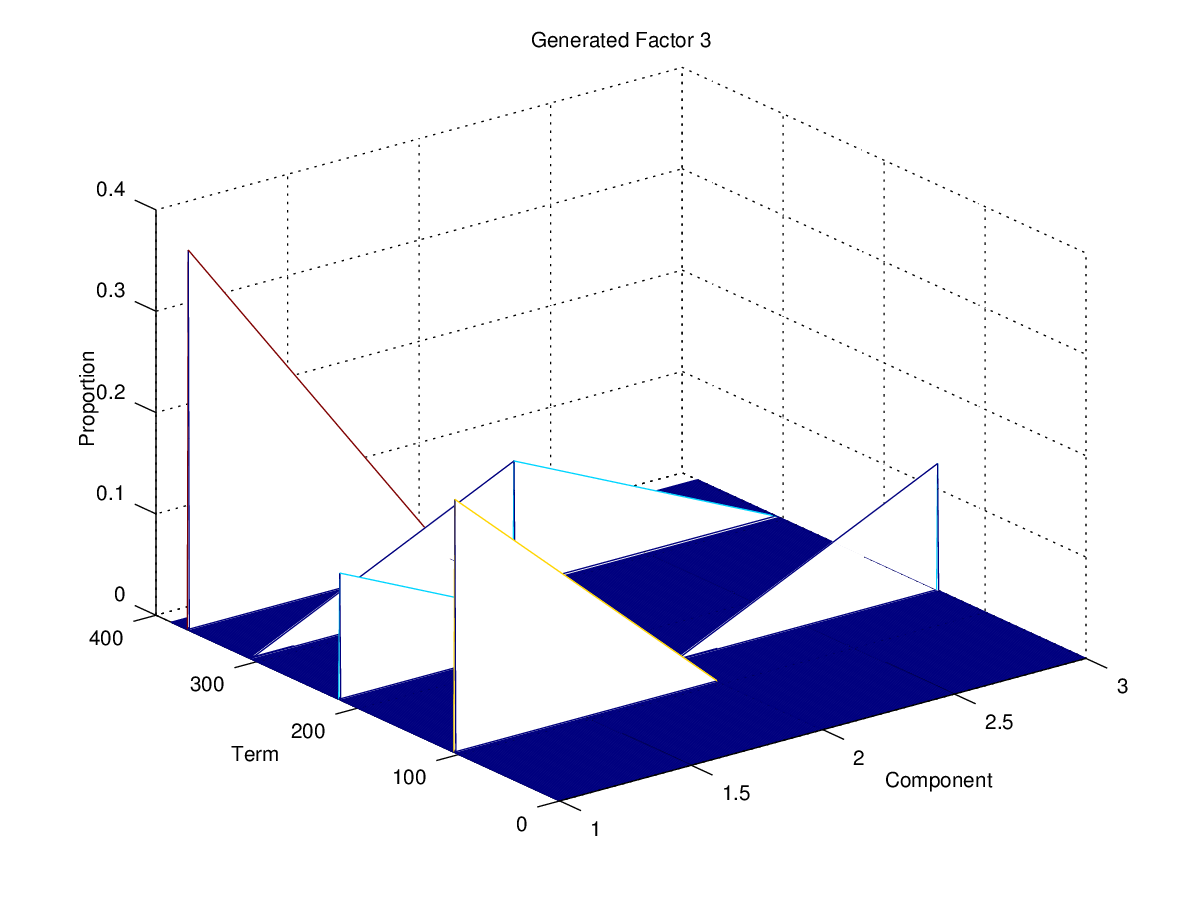
\includegraphics[width=0.4\textwidth]{plots/gen3} }}%
    \qquad
    \subfloat{{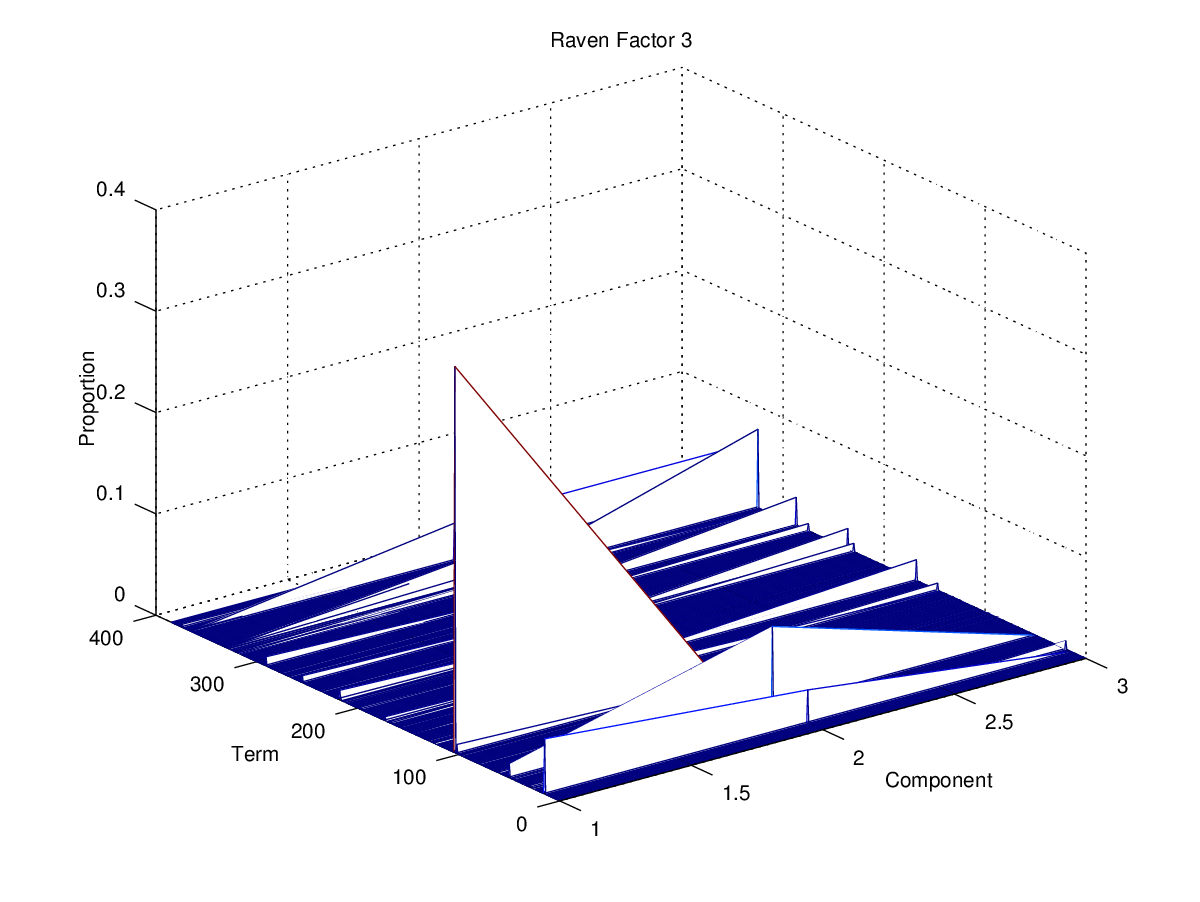
\includegraphics[width=0.4\textwidth]{plots/rav3}
    }}%
    \caption{Factor 3 Match}%
    \label{fig:com3}%
    Influence Source: Raven Factor 3 
    \par Influence Weight = 0.12
\end{figure}
\end{frame}

\begin{frame}{Factor 4 Match}
\begin{figure}%
    \centering
    \subfloat{{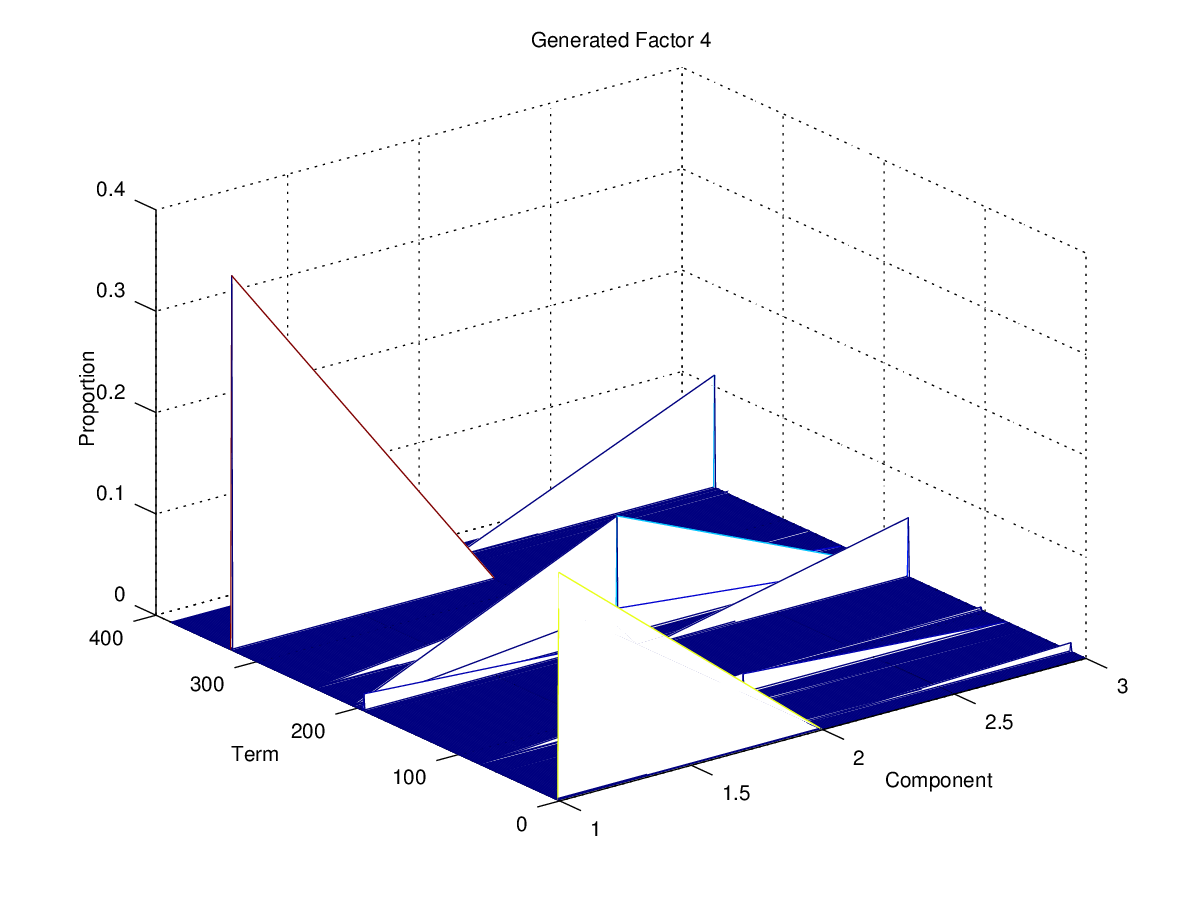
\includegraphics[width=0.4\textwidth]{plots/gen4} }}%
    \qquad
    \subfloat{{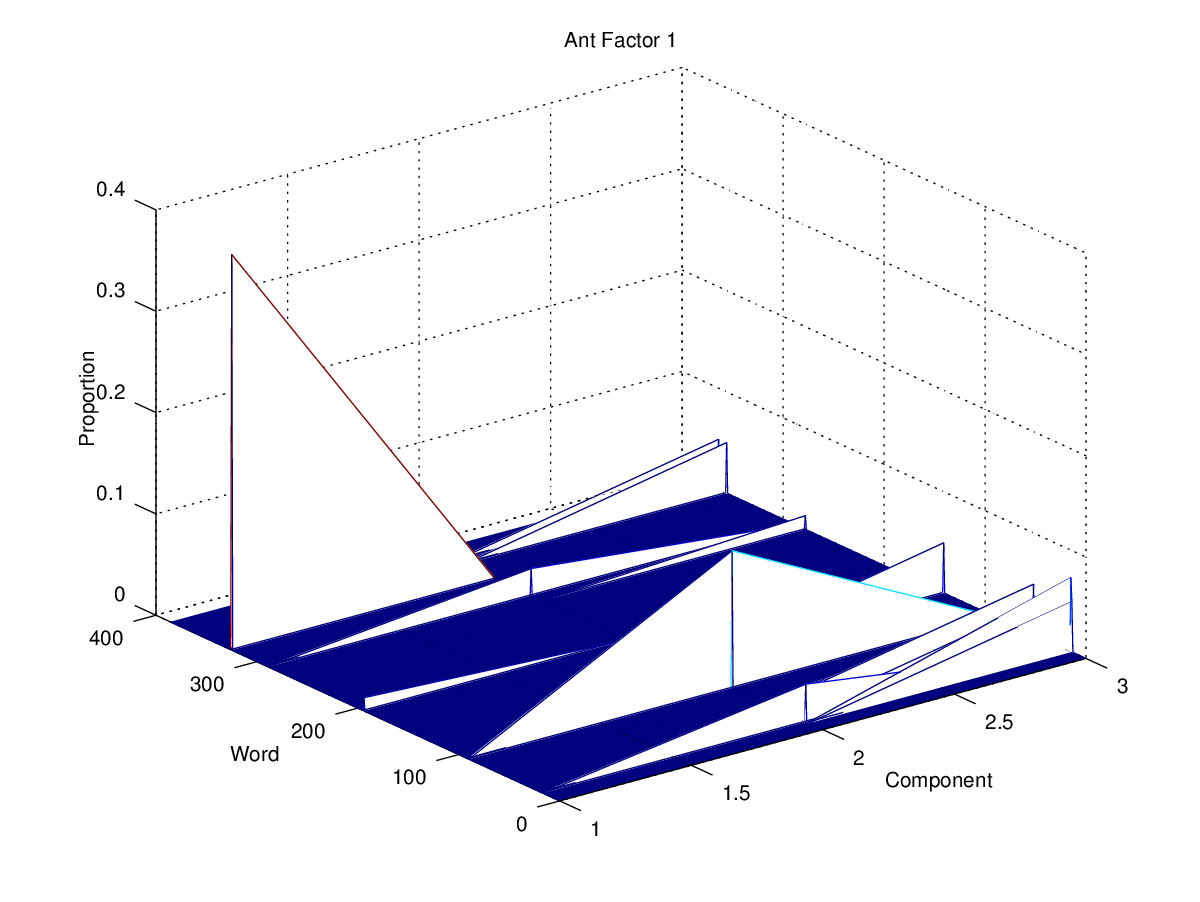
\includegraphics[width=0.4\textwidth]{plots/ant1}
    }}%
    \caption{Factor 4 Match}%
    \label{fig:com4}%
    Influence Source: Ant Factor 1 
    \par Influence Weight = 0.14
\end{figure}
\end{frame}

\begin{frame}{Factor 5 Match}
\begin{figure}%
    \centering
    \subfloat{{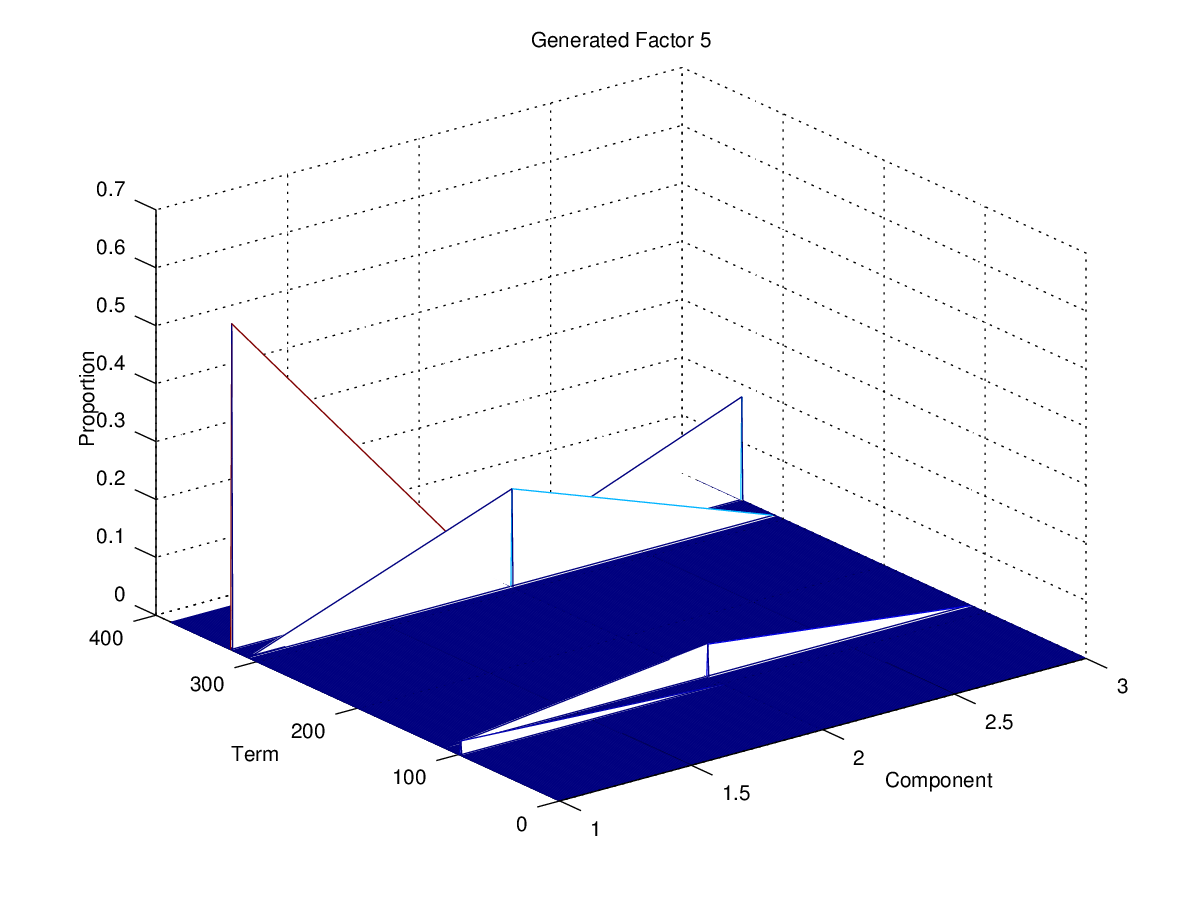
\includegraphics[width=0.4\textwidth]{plots/gen5} }}%
    \qquad
    \subfloat{{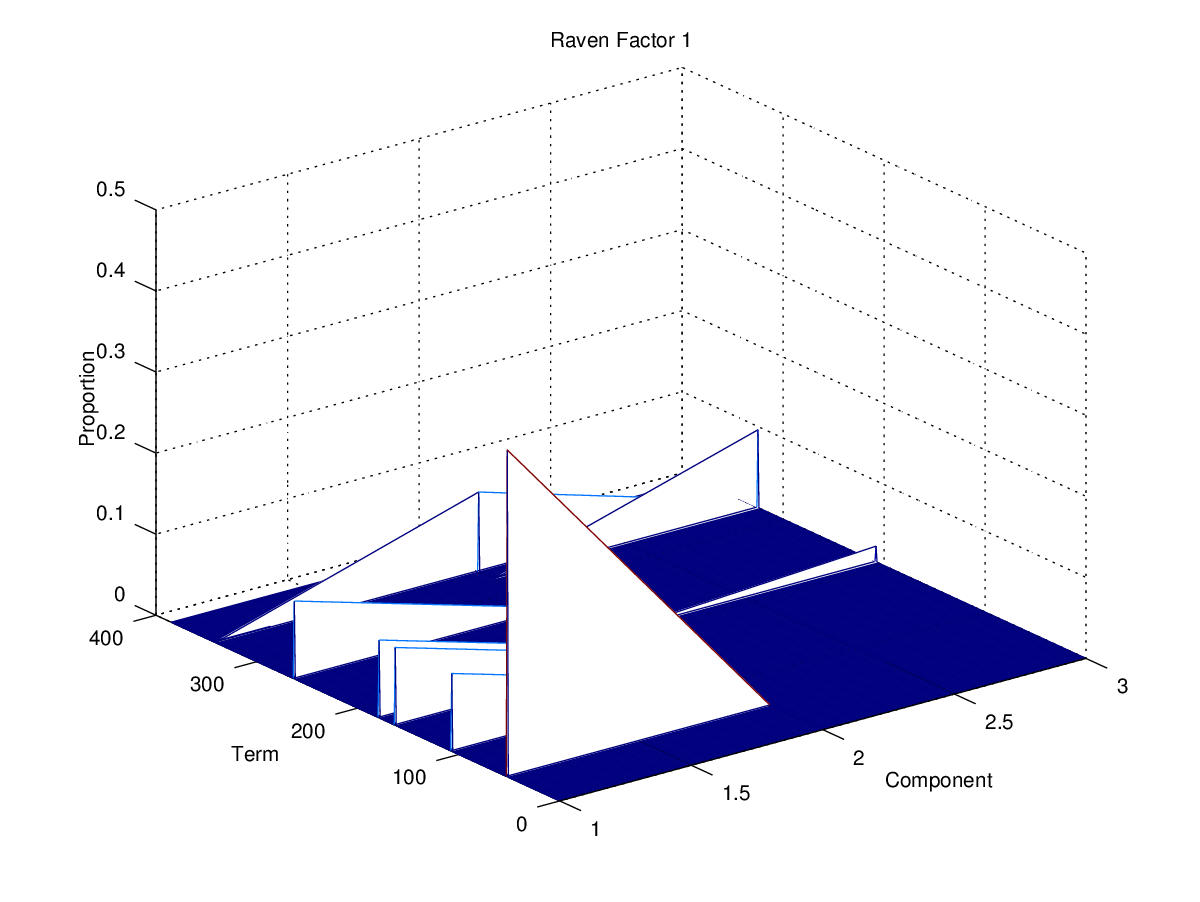
\includegraphics[width=0.4\textwidth]{plots/rav1}
    }}%
    \caption{Factor 5 Match}%
    \label{fig:com5}%
    Influence Source: Raven Factor 1 
    \par Influence Weight = 0.10
\end{figure}
\end{frame}


\section{Future Work and Contributions}
\begin{frame}{Influence Model Contributions}
    \begin{itemize}[<+->]
        \item Better factor comparisons are needed.
        \item Statistics which account for multiple factor contributions to citing factors are needed.
        \item Validation techniques need to be developed.
    \end{itemize}
\end{frame}

\begin{frame}{Filtering}
    \begin{itemize}[<+->]
        \item Some topics and phrasings will be common to many documents.
        \item Assertions of origins of ideas and contributing factors necessitate filters of common phrases.
        \item Stylistic influence modelling may be possible given commonality filtering.
    \end{itemize}
\end{frame}

\begin{frame}{Software Contributions}
    \begin{itemize}[<+->]
        \item The software used for these decompositions was Rasmus Bro's n-way toolkit~\cite{andersson2000}
        \item Existing tensor packages cannot handle the size of real-world tensors.
        \item For example, the papers cited in the present proposal comprise a 20,000 word vocabulary!
        \item Robust sparse tensor tools are needed.
        \item The results will be released as open source software.
    \end{itemize}
\end{frame}

\begin{frame}{Extensions and Applications}
    \begin{itemize}[<+->]
        \item Topological sorting to determine document chronology.
        \item Identification of uncited influential documents in a corpus.
        \item Modelling of transitive influence.
    \end{itemize}
\end{frame}

\begin{frame}[allowframebreaks]{Bibliography}
\setbeamertemplate{bibliography item}{\insertbiblabel}
\bibliography{sources}{}
\bibliographystyle{plain}
\end{frame}

\end{document}


